\documentclass[12pt]{article}
\usepackage[paper=a4paper,left=25mm,right=25mm,top=25mm,bottom=25mm]{geometry}
\usepackage[english]{babel}
\usepackage[utf8]{inputenc}
\usepackage[pdftex]{graphicx}
\usepackage{tikz-qtree}
\usepackage{color}
\usepackage{amssymb}
\usepackage{amsthm}
\usepackage{hyperref}
\usepackage{enumitem}
\usepackage{pdfpages}
\usepackage{hyperref}
\usepackage{subcaption}


\linespread{1.25}

\begin{document}
\tikzset{every tree node/.style={minimum width=2em,draw,circle},
         blank/.style={draw=none},
         edge from parent/.style=
         {draw,edge from parent path={(\tikzparentnode) -- (\tikzchildnode)}},
         level distance=1.5cm}
\begin{titlepage}

\includegraphics[height=20mm]{images/uzh_logo}\\

\begin{flushleft}

\vspace{2cm}

{\Large Introduction to Artificial Intelligence\\Exercise Sheet 6}\\

\vspace{4cm}

\textbf{Laurin van den Bergh, 16-744-401\\Yufeng Xiao, 19-763-663\\Nora Beringer, 19-734-227}\\

\vspace{2cm}

Universität Zürich\\
Institut für Informatik

\vfill Due: April 06, 2022

\vspace{3cm}


\end{flushleft}
\end{titlepage}

\newpage

\section*{Exercise 6.1}
a) We first brought $\varphi$ into CNF in order to make e decision about the propositional formula in Task 6.1 a). Please consider the justification down below.\\
b) \\
$\varphi = \lnot (A \to (B \land \lnot C)) \land ((A \land C ) \lor \lnot B)$\\
$\varphi \equiv \lnot (\lnot A \lor (B \land \lnot C)) \land ((A \land C) \lor \lnot B)$ \qquad Implication eliminiation\\
$\varphi \equiv A \land \lnot (B \land \lnot C) \land ((A \land C) \lor \lnot B)$ \qquad DeMorgan Law, Double Negation eliminiation\\
$\varphi \equiv A \land \lnot (B \land \lnot C) \land (A \lor \lnot B) \land (C \lor \lnot B)$ \qquad Distribution Law\\
$\varphi \equiv A \land (\lnot B \lor C) \land (A \lor \lnot B) \land (C \lor \lnot B)$ \qquad DeMorgan Law\\
$\varphi \equiv A \land (A \lor \lnot B) \land (C \lor \lnot B)$\qquad remove duplicate sentence\\ \\
Justification for a):\\
Set A to true and C to true then $\varphi$ is satisfiable, hence it is not unsatisfiable.\\
Set A to false then $\varphi$ is not valid.\\
Because the sentence $\varphi$ is satisfiable and not valid it is falsifiable.


\section*{Exercise 6.2}
a)\\
$\varphi \vDash \psi$\\
$\psi = C \land \neq D, \neq \psi \equiv \neq C \lor D$\\
Test if $\varphi \to \psi$ is a tautology,\\
equivalently: test if $\psi \cup \{\neq \psi \}$ is unsatisfiable =: $\Delta$, where $\Delta$ is in CNF.\\
Consider the Resolution steps down below:\\ \\
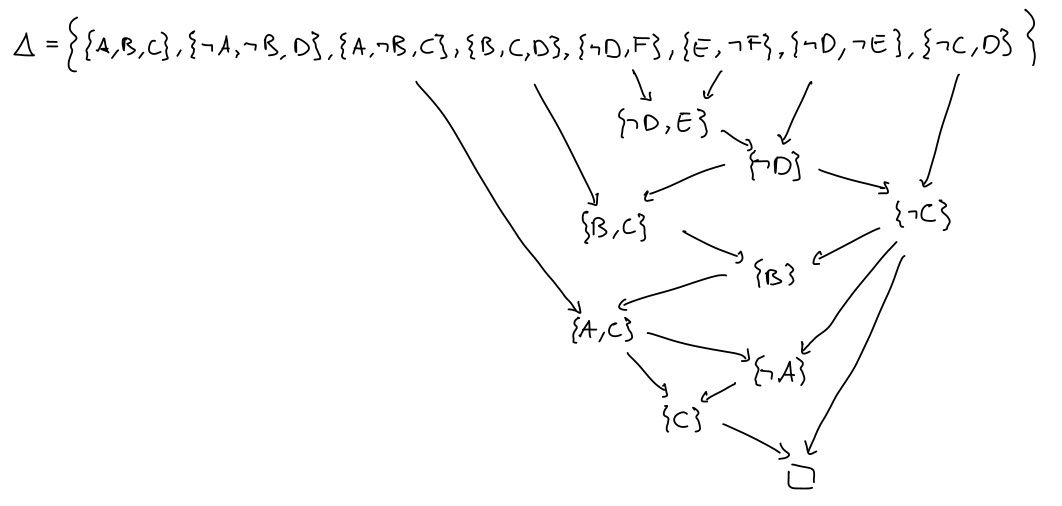
\includegraphics[height=90mm]{images/6.2a}\\
b) We used 9 steps. A truth table for the same sentence would have 2$^6$ rows as the number of variables (A, B, C, D, E, F) is equal to 6. Therefore we need less steps for the Resolution in comparison tho building the truth table.\\


\section*{Exercise 6.3}
a)\\
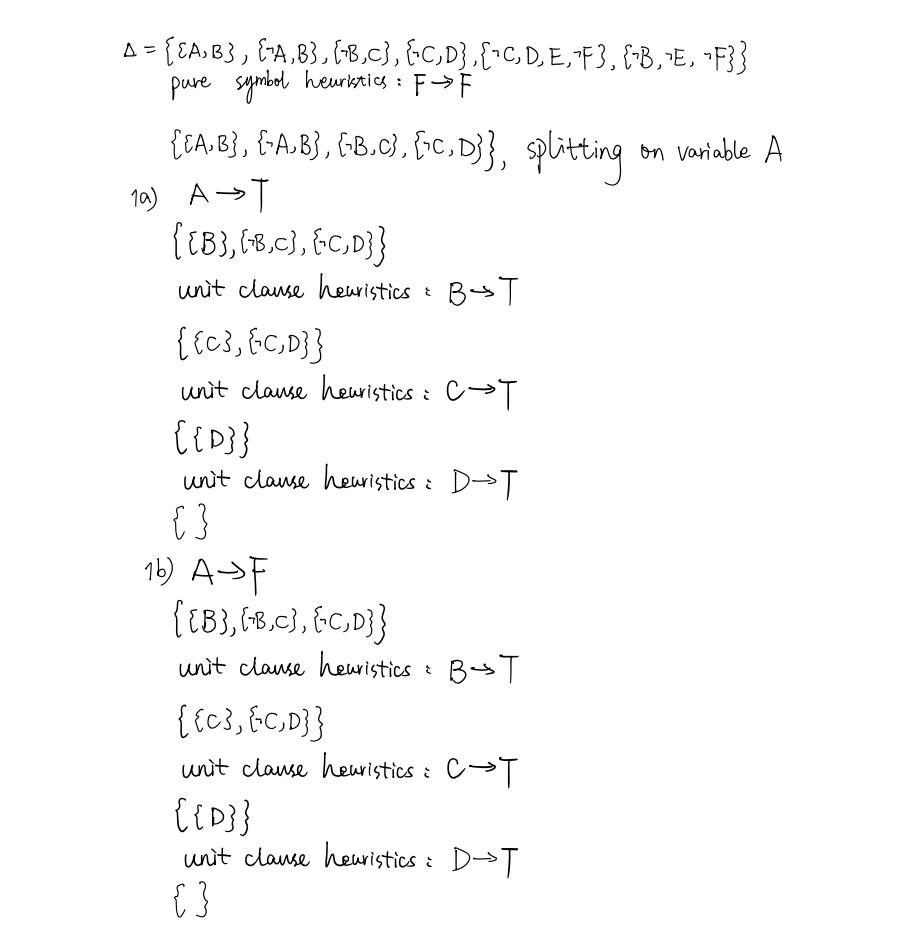
\includegraphics[height=100mm]{images/6.3a}\\

\section*{Exercise 6.4}
a) As we didn't find a pure symbol or unit clause heuristic we choose to split on A, while assigning True first for splitting. We then break ties in alphabetical order.\\
Leading to the following recursive structure of 1a):\\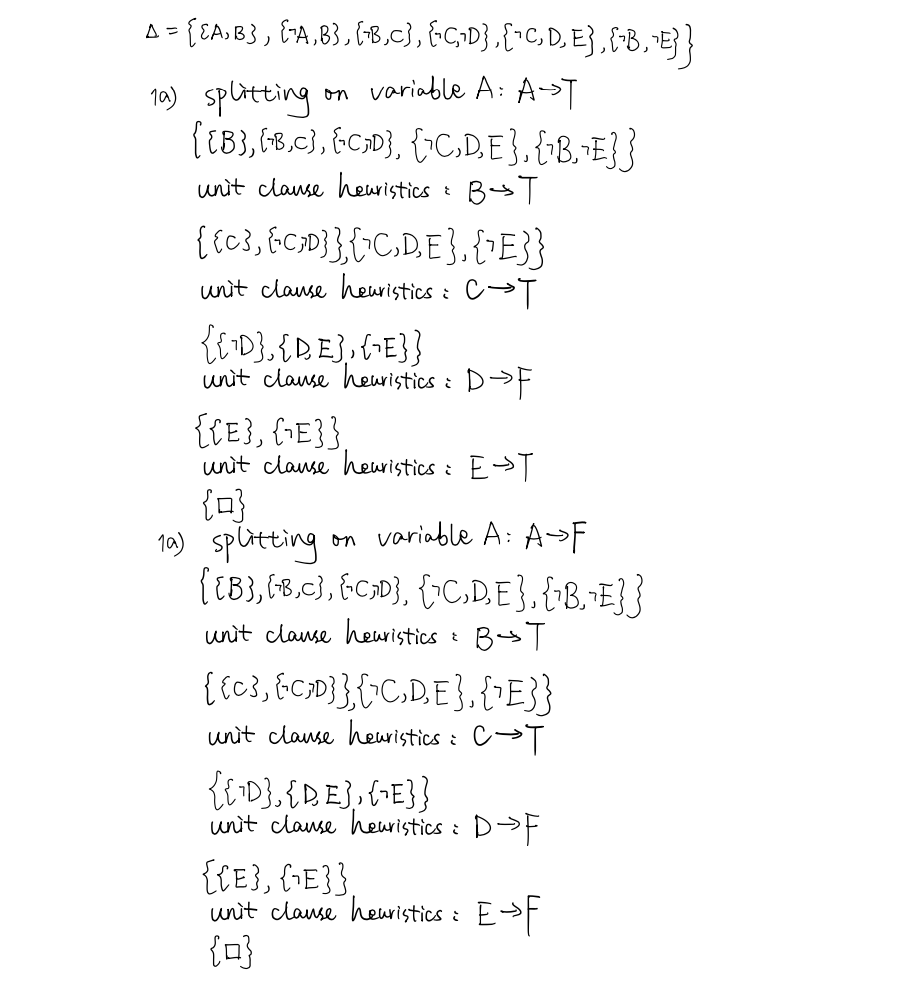
\includegraphics[height=100mm]{images/6.4}\\
b) The variable order doesn't influence the DPLL execution in this example. Whichever variable we choose for splitting, while afterwards picking True first, will lead to the same amount of steps as demonstrated in 6.4 a)\\
c) When we take the variable order used in 6.4 a) and pick False first we still have the same amount of steps until the DPLL terminates. Hence the Termination will be reached at the same speed. This is because after the first Iteration where we split on Variable A, where A $\to$ F, we end up with a the unsatisfied clauses where we have to choose the unit clause heuristic for B next, where B $\to$ T. Afterwards the order will be the same as in a) if we follow the breaking of ties in alphabetical order. We have provided the recursive structure as well under 6.4a) 1b).\\

\end{document}